\documentclass[11pt]{article}
%Gummi|065|=)
\usepackage{graphicx}
\title{\textbf{Práctica 3 - IG}}
\author{Javier Sáez Maldonado}
\date{}
\begin{document}

\maketitle

\section{Modelo jerárquico}

En nuestro modelo jerárquico, he tratado de representar una persona que se mueve a la vez que toca una pequeña batería, mueve sus brazos y agita su cabeza y sus piernas, a la vez que se mueve el platillo de la batería.

\section{Grados de Libertad}
Los parámetros tienen la misma velocidad inicial, incremento y aceleración. Hay 6 grados de libertad:
\begin{itemize}
	\item Movimiento de uno de los brazos del muñeco. Este es una rotación vertical respecto del eje X, acotado, con valor inicial 20, semiamplitud 10 y frecuencia 0.5.
	\item Movimiento del otro brazo del muñeco. Este es una rotación  respecto del eje Z, acotado, con valor inicial 20, semiamplitud 15 y frecuencia 0.5.
	\item Movimiento de la cabeza del muñeco. Este es una rotación vertical respecto del eje X, acotado, con valor inicial 20, semiamplitud 40 y frecuencia 0.2.
	\item Movimiento del platillo. Este es una rotación vertical respecto del eje X, acotado, con valor inicial 20, semiamplitud 10 y frecuencia 0.4.
	\item Movimiento de una de las piernas del muñeco. Este es una rotación vertical respecto de los ejes Y y Z, acotado, con valor inicial 20, semiamplitud 10 y frecuencia 0.5.
	\item Movimiento de una de las piernas del muñeco. Este es una rotación vertical respecto de los ejes X,Y y Z, acotado, con valor inicial -20, semiamplitud -10 y frecuencia 0.5.
\end{itemize}

\section{Grafo PHIGS}
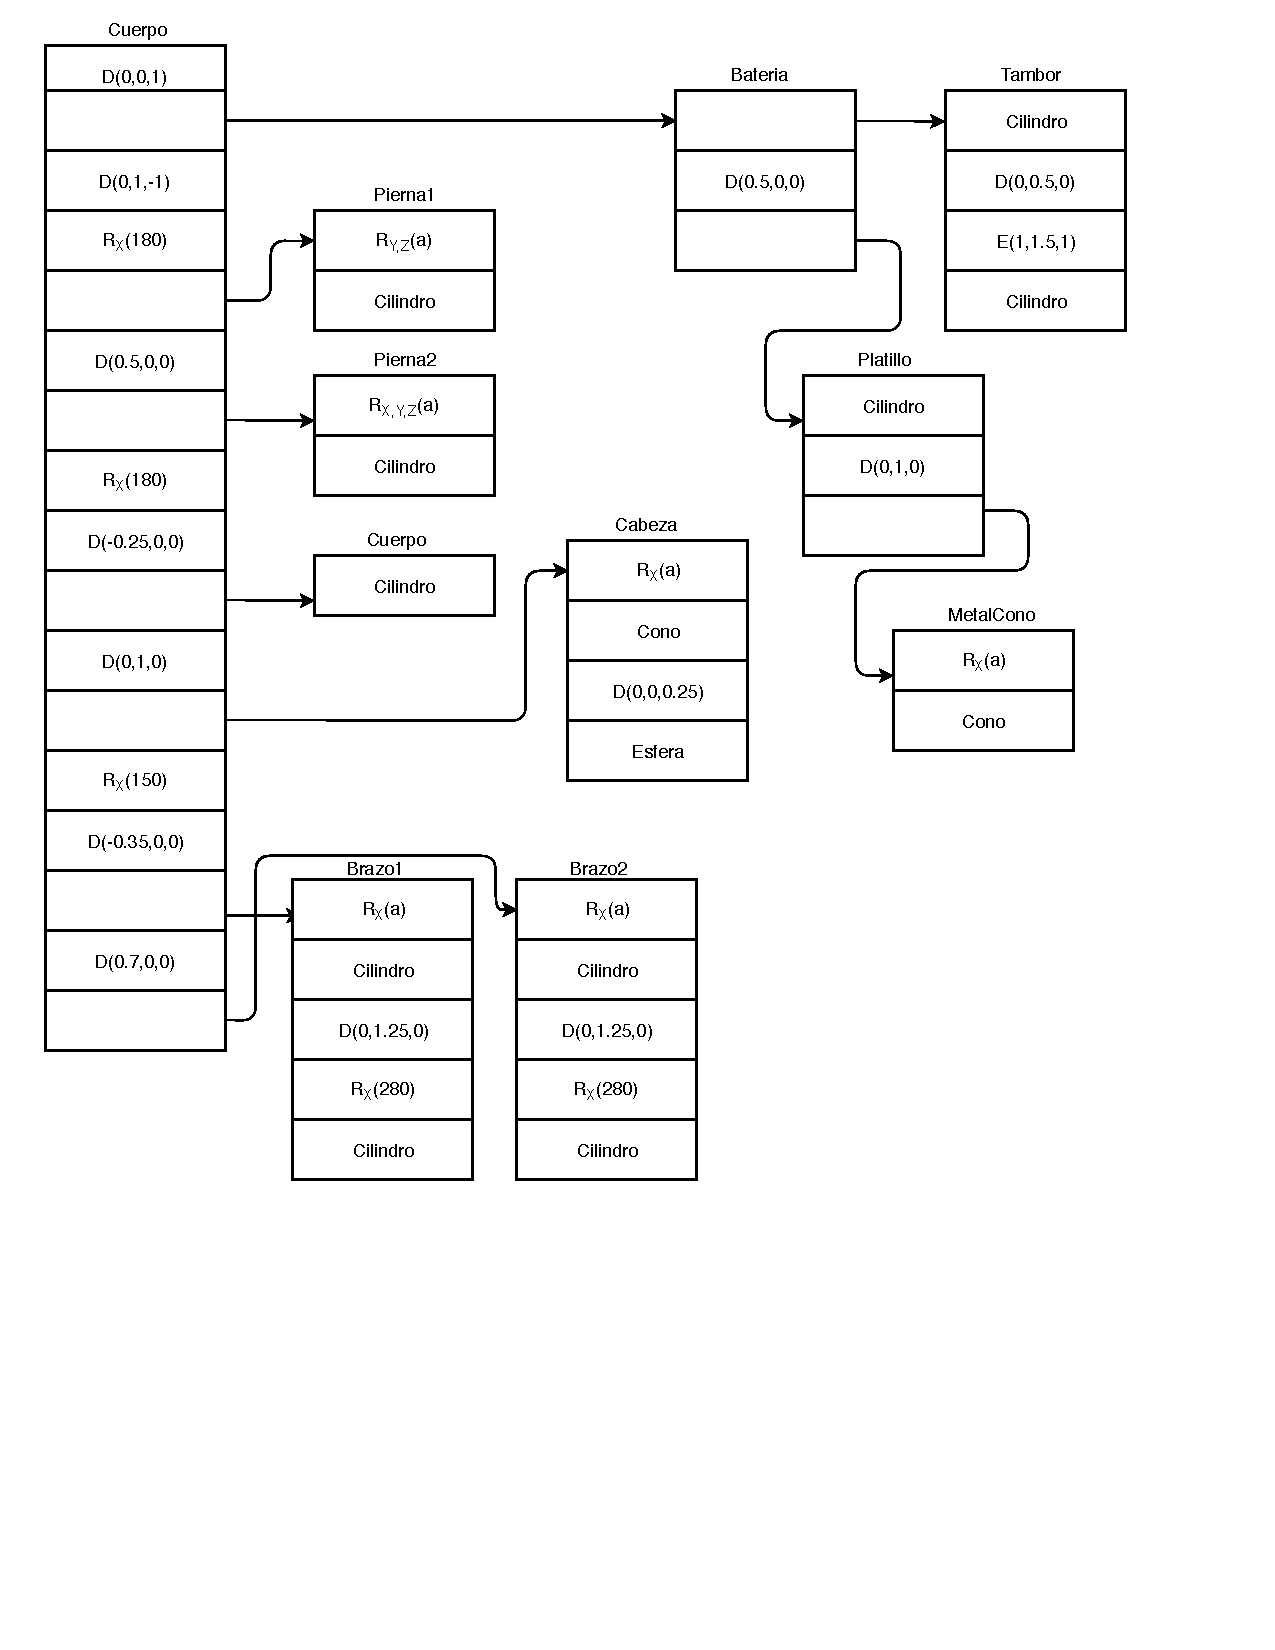
\includegraphics[scale=0.8]{PHIGS.pdf}

\end{document}
